\section{性能試験}
製作した力覚センサに対する性能試験の結果について述べる. 

製作した力覚センサをFig.~\ref{fig:jissai}に示す.

\begin{figure}[h]
  \centering
  \subfloat[低剛性起歪体]{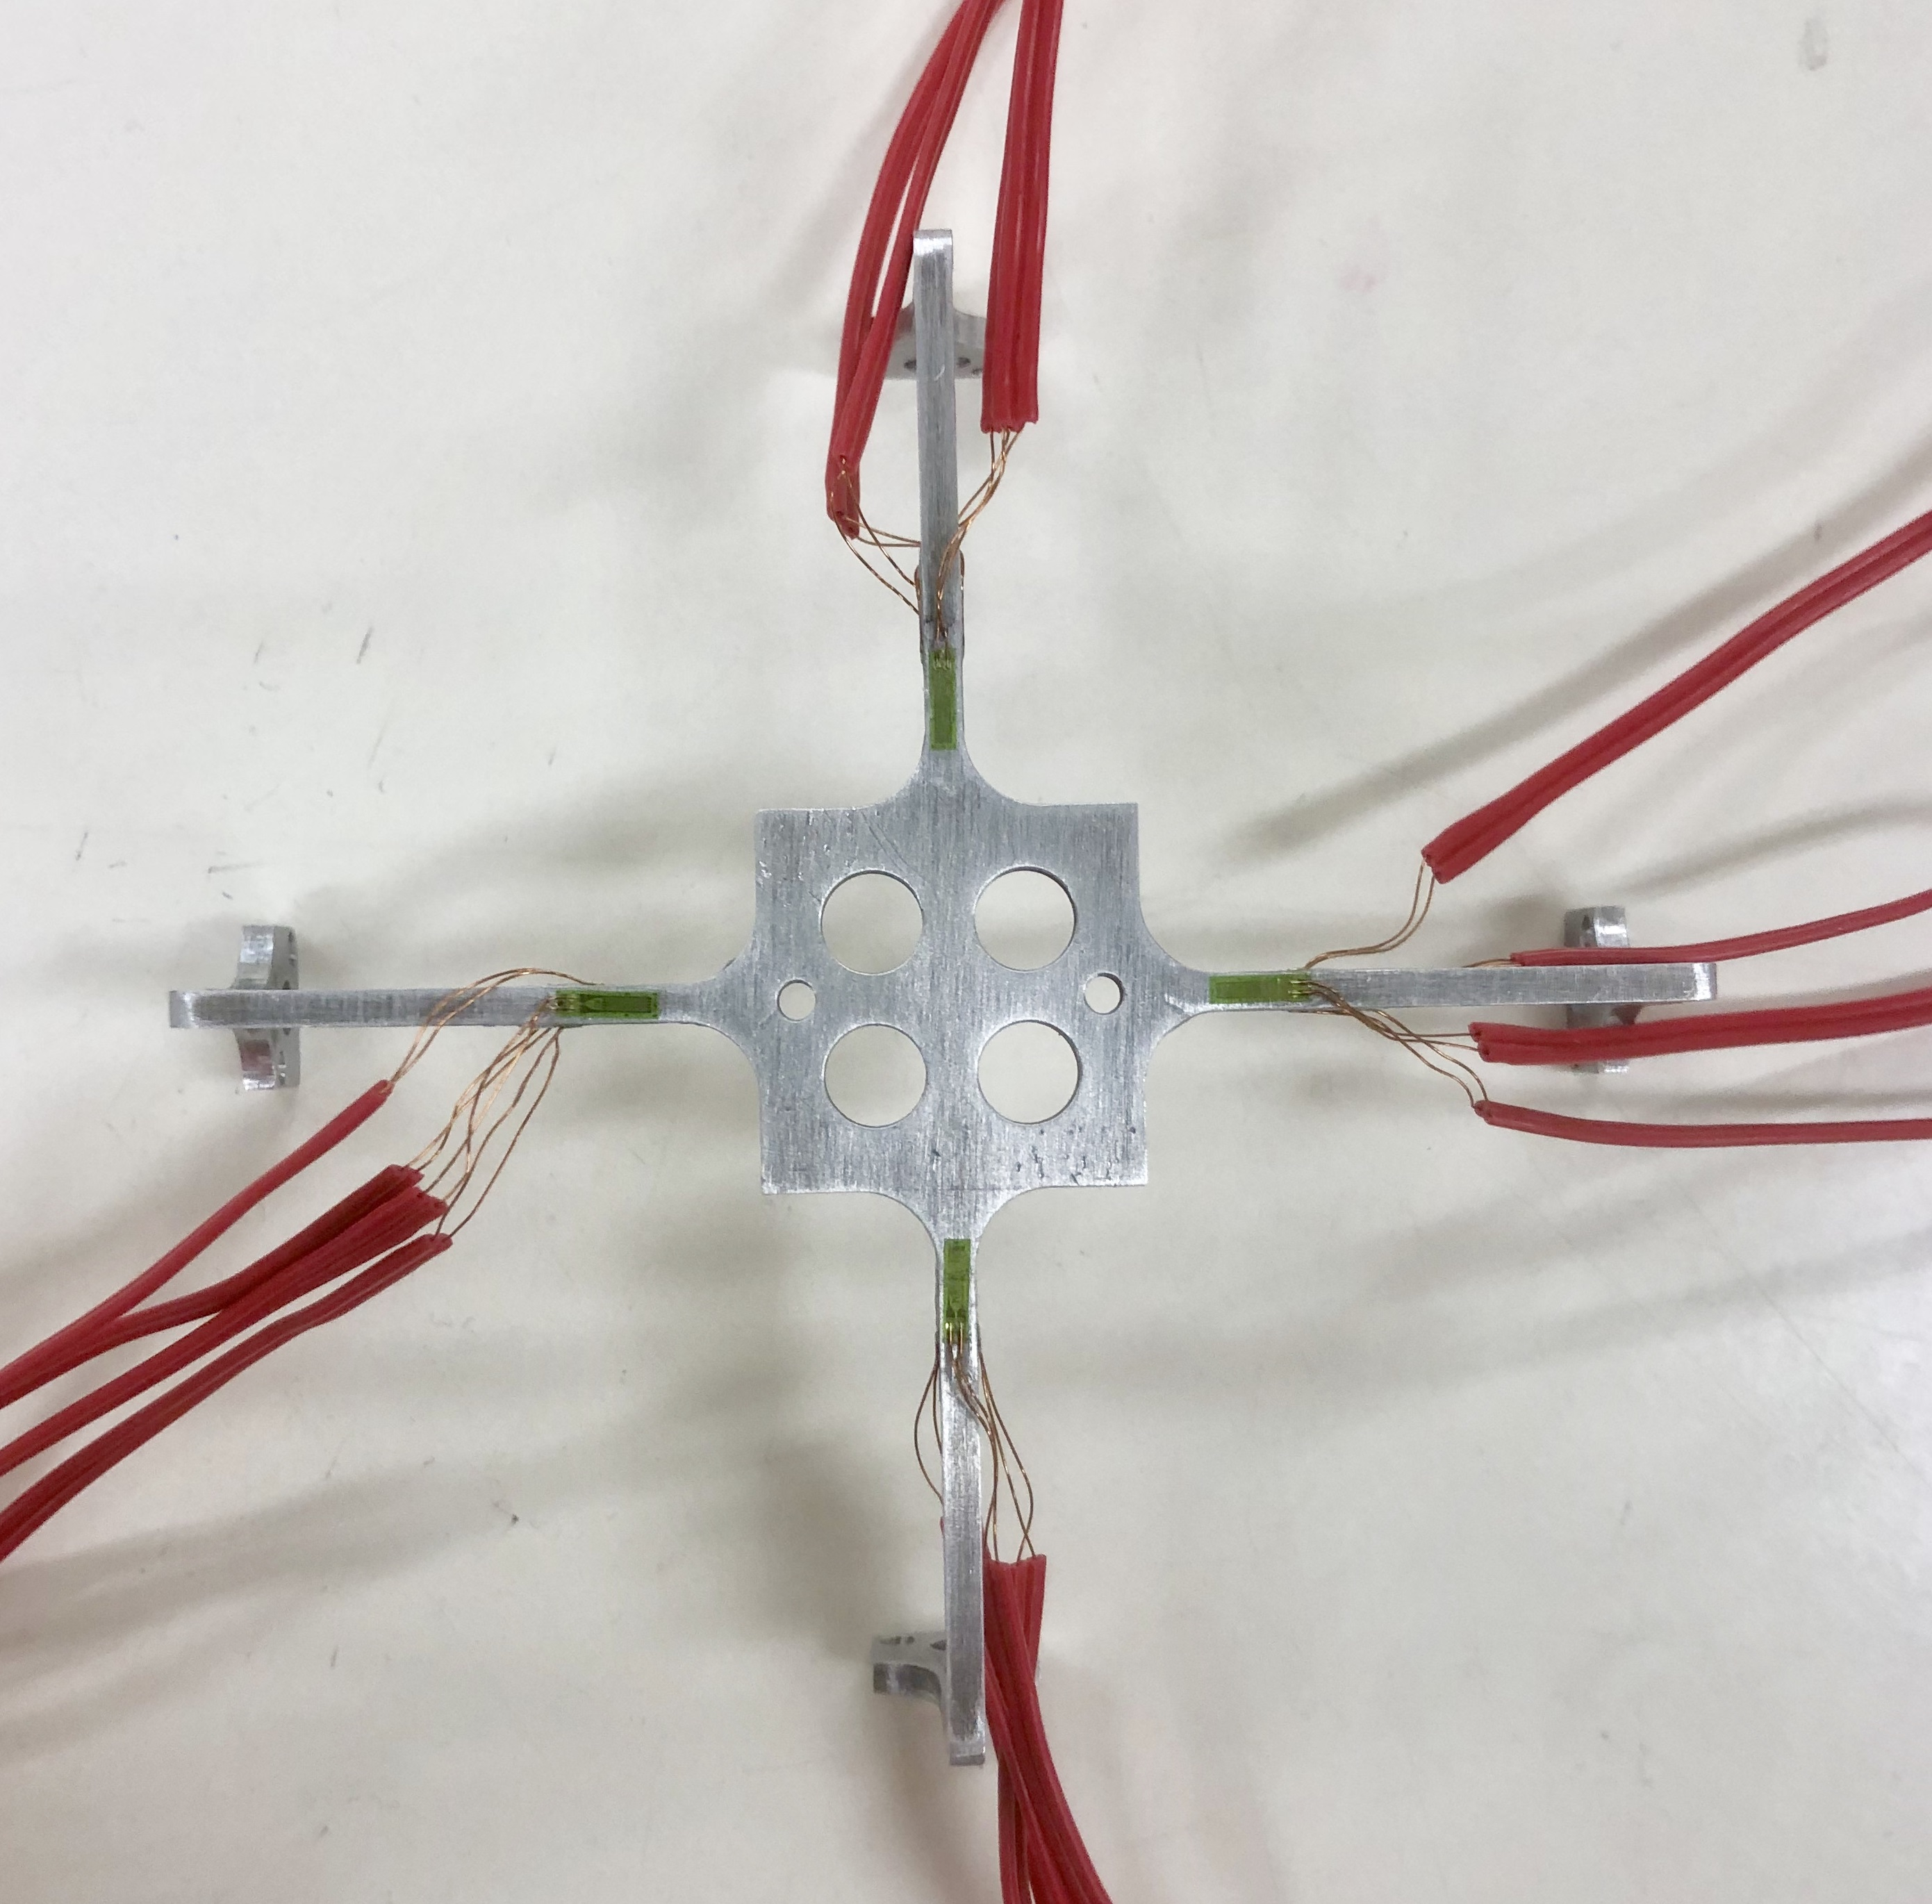
\includegraphics[width=4.2cm]{pic/real_L.jpg}}
  \subfloat[高剛性起歪体]{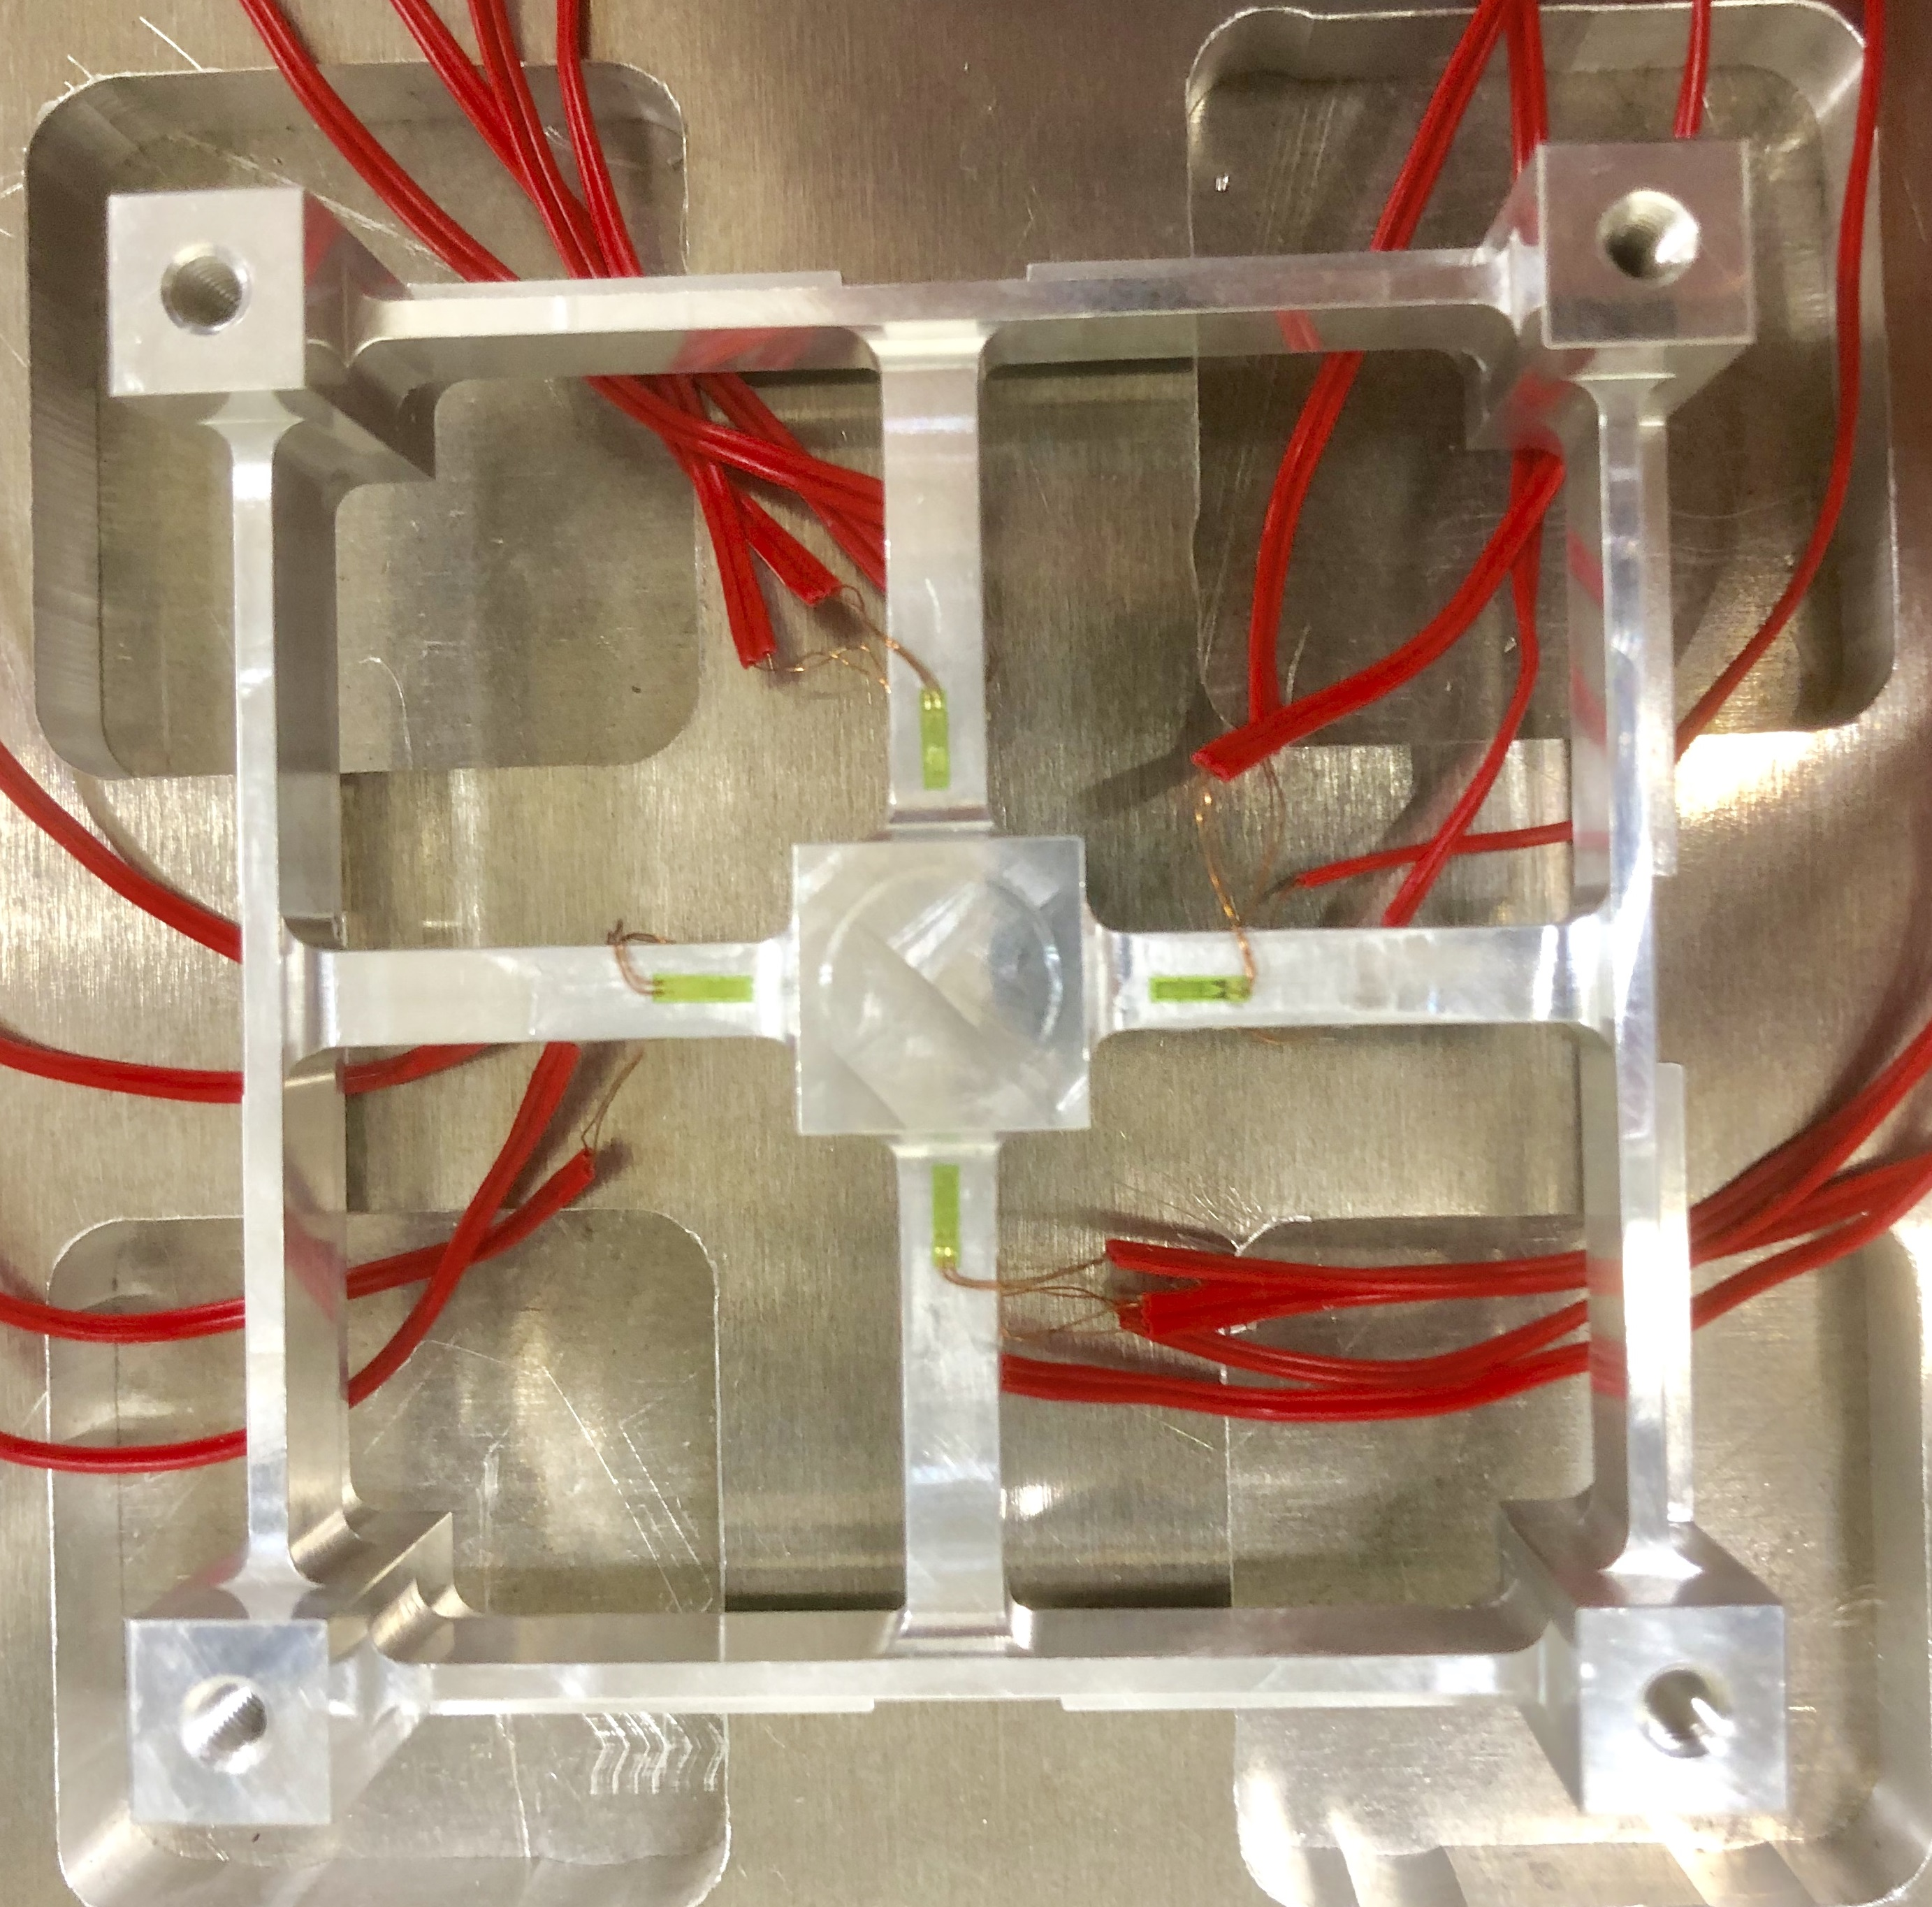
\includegraphics[width=4.2cm]{pic/real_H.jpg}}\\
  \caption[]{製作した小型HDR6軸力覚センサ}\label{fig:jissai}
\end{figure}

\subsection{非線形性・他軸干渉試験}
力覚センサは荷重-ひずみ変換行列を用いて印加荷重を算出する. 
印加された荷重に対する出力値の非線形性や, 
印加された荷重以外の成分の出力が応答する他軸干渉は
力覚センサの性能に関わる重要な指標である. 
 

算出した荷重-ひずみ変換行列により変換した低剛性起歪体の荷重出力を
Fig.~\ref{fig:kajyuLow}に示す.
6軸ともに線形的な出力結果が得られた. 
しかし, $F_x, F_z, M_z$の結果を見ると, 他軸干渉成分が較正しきれていないことが
確認できる. 

%\begin{eqnarray}
%  NL^{F_x} = \frac{L^{F_x}_{true} - L^{F_x}_{out}}{L^{F_x}_{rated}}
%\end{eqnarray}

%\begin{eqnarray}
%  \scalebox{0.7}{$\displaystyle
%  CC^{F_x} = \sqrt{\Biggl(\frac{L^{F_y}_{out}}{L^{F_y}_{rated}}\Biggr)^2 + \Biggl(\frac{L^{F_z}_{out}}{L^{F_z}_{rated}}\Biggr)^2 + \Biggl(\frac{L^{M_x}_{out}}{L^{M_x}_{rated}}\Biggr)^2 + \Biggl(\frac{L^{M_y}_{out}}{L^{M_y}_{rated}}\Biggr)^2 + \Biggl(\frac{L^{M_z}_{out}}{L^{M_z}_{rated}}\Biggr)^2}
%$}
%\end{eqnarray}
%ここで, $L_{true}$は印加荷重の真値, $L_{out}$はセンサ出力, $L_{rated}$は定格荷重, 上添え字は6成分を表す. 

低剛性起歪体は$M_y$以外の軸では算出結果からも線形性が示された. 
高剛性起歪体は低剛性起歪体と比較すると非線形的であるが, 
Fig.~\ref{fig:kajyuHigh}で確認できた結果同様に$F_z, M_y$以外の軸は
線形性が示された. また他軸干渉においては低剛性起歪体の結果が
大きい数値を示している. これは主軸自体の出力値が小さい分, 
他軸成分が大きく干渉してしまっていると考えられる. 

\subsection{SN比と測定レンジ}
Fig.~\ref{fig:sn}に各ひずみゲージから得られた出力のSN比の推移を示す. 
この結果は高周波ノイズ(0.3\%R.O.), 非線形性, 他軸干渉を考慮したものとなっている. 


この結果より, 1つの起歪体上に種類の異なるひずみゲージを張り付けることで
1つのセンサとして力の測定が可能なことが分かる.  
よって本力覚センサは0.2Nから500Nの測定レンジを有していることが示された.